\section{Entrepôts de données}\label{sec:rw:supervision:warehouse}
Pilier de l'informatique décisionnelle (\textit{Business Intelligence}), l'approche par entrepôt de données (\textit{Data Warehouses}) est très réputé et grandement répendue. Son apport est originellement utilisé dans les applications pour entreprises. Toutefois sa capacité de traitement et ses outils d'analyses visuels ont permit son introduction dans d'autres cœurs de métiers tels que les réseaux~\cite{refneeded} ou l'agriculture~\cite{Abdullah:olap}. Cette architecture a été prévue pour permettre de fournir des outils d'analyses de données puissants. Pour cela, des procédés ont étés développés pour permettre de faire de l'intégration de données hétérogènes, ainsi que des structures d'entrepôts prêts à répondre aux besoins d'analyses.

Son impact dans le cadre de la supervision semble clair. En effet, puisque l'observation et la compréhension du système passe par son analyse, des outils sont nécessaires pour effectuer ces opérations. L'établissement de diagnostic nécessite effectivement le parcours des données pour mieux comprendre les causes d'un problème. De plus, sa structure permettant l'intégration de donnée est à considérer pour intégrer les sources de données auxquelles nous sommes confrontés.

Par la suite, cette section détaille en premier lieu l'architecture globale de la solution. Nous détaillerons ensuite comment l'intégration est faite via les processus \textit{ETL}. Ensuite nous décrirons les structures de données utilisées pour permettre différentes analyses. Enfin, nous présenterons brièvement quelques outils d'analyses pouvant raisonner sur les données.

\subsection{Architecture globale}
La définition fonctionnelle d'un entrepôt de donnée est \enquote{\it une collection de données orientées sujet, intégrées, non volatiles et historisées, organisées pour le support d’un processus d’aide à la décision}~\cite{Inmon:warehouse}. Au sens large, un entrepôt est une base de donnée avec une organisation qui s'oriente avant tout sur l'application finale (l'analyse) plutôt que sur l'intégrité des données, et qui refuse la suppression ou la modification de données afin de garder une trace.
\begin{figure}[ht]
	\centering
	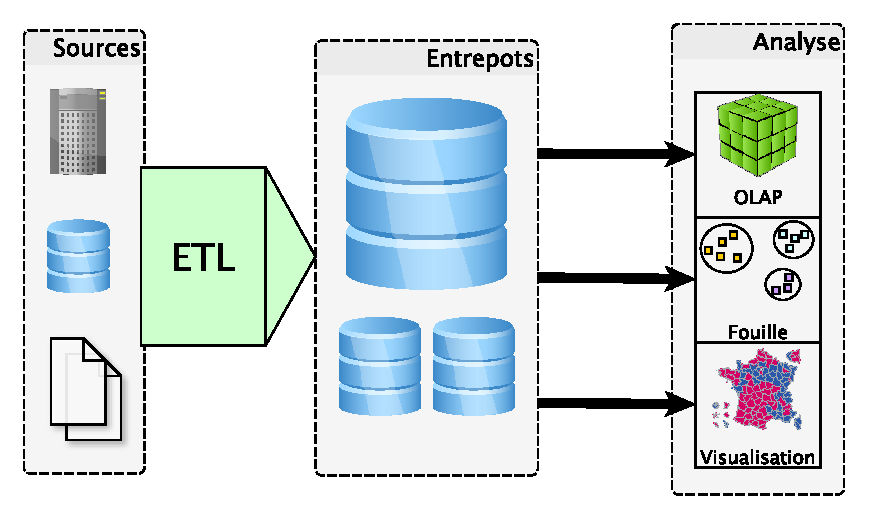
\includegraphics[width=0.75\textwidth]{rw-supervision-warehouses}
	\caption{Architecture globale d'une solution d'entrepôts de données}\label{fig:rw:supervision:warehouses}
\end{figure}
La figure~\ref{rw-supervision-warehouses} présente une architecture abstraite des approches à entrepots. Les données sources sont supposées être dans des bases de données opérationnelles au mieux, ou à l'intérieur de fichier brute, au pire. A partir de ce constat, il est acté que les sources sont donc hétérogènes autant en terme de syntaxe ou de sémantique.

Afin d'effectuer l'intégration des données à l'intérieur d'un (ou des) entrepôt(s), il faut traiter cette hétérogénéité et charger les données. Les processus \textit{ETL} ont été conçus pour cette tâche. Ces procédés sont découpés en trois phases : l'extraction (\textit{\textbf{E}xtract}), le traitement (\textit{\textbf{T}ransform}) et enfin le chargement (\textit{\textbf{L}oad}). Cet aspect sera détaillé en section~\ref{sec:rw:supervision:warehouse:etl}.

Par la suite, des outils d'analyses vont s'attacher aux entrepôts pour fournir les informations suffisantes à l'utilisateur pour qu'il puisse prendre une décision. Comme montré dans la définition des entrepôts, les bases de données sont conçus pour que ces outils d'analyses puissent effectuer leurs calculs nativement. La structure interne des entrepôts aura donc un impact sur la capacité des outils d'analyse.

\subsection{L'entrepôt et ses capacités}\label{sec:rw:supervision:warehouse:warehouse}
Les dépots de données ont pour but de stocker toutes les données relatives à un système. Son système de gestion est très souvent fait par un SGFD relationnel\footnote{Il est évident que des systèmes de gestion dédiés soient choisis pour des critères de performances}. C'est sa structure et ses opérations qui vont permettre une analyse pertinente.

Le cadre le plus récurrent pour les entrepôts de données est le traitement OLAP (\textit{Online Analytical Processing}). 
\subsubsection{OLAP}
Le terme \textit{OLAP} a été d'abord défini en 1993 par le père du modèle relationnel, Edgar Codd, dans~\cite{Codd:olap}. Sa caractérisation est le fait de permettre le support \textit{d'analyse de données multidimensionnelles}. En effet, il apparait qu'une donnée représente un point dans un espace à plusieurs dimensions. L'exemple le plus standard dans ce domaine reste la gestion de vente pour une entreprise. La vente est un point dans l'espace $(Magasin, Produit, Temps)$ et sa valeur sera le prix (et/ou la quantité). L'analyse de ces données sur ces trois critères requiert des capacités spécifiques pour que l'analyse soit pertinente.

En 1995, les premiers concepts d'opérations multidimensionnelles arrivent avec le \textbf{cube}~\cite{Gray:cube}. Les dimensions doivent être définies de manière hiérarchique. Par exemple, un magasin (lieu) est située dans une ville, elle-même située dans un département, elle même située dans une région etc.. Par la suite, le traitement sur les données en elle-même va être centré sur la capacité à faire un agrégat. Dans notre cas, il est potentiellement intéressant de voir les résultats de vente par départements. Une somme est ainsi faite sur tous les résultats de chaque département.

L'hypercube \textit{OLAP} est la représentation des données multidimensionnelles. Dans notre cas, cela va être un vrai cube à trois dimensions, les magasins, les produits, et le temps. Au début de l'analyse les dimensions sont discrétisé à leur plus haut niveau hiérarchique.
\begin{figure}[ht]
	\centering
	\TODO{}
	\caption{Représentation d'un cube \textit{OLAP} de trois dimensions, $(Magasin, Produit, Temps)$}
\end{figure}
Cela forme un découpage du cube en autres cubies. Chacun de ces cubies contient la valeur d'un ou plusieurs agrégats choisis par l'utilisateur (ici, \textit{SUM}). Il est important de dire que l'utilisateur ne pourra pas que rarement exploiter correctement les $n$ dimensions de l'hypercube, car la représentation classique des données est sous forme de tableaux (donc 2 dimensions). Plusieurs opérations génériques existent sur ce cube pour que l'utilisateur puisse l'exploiter.

\subsubsection{Opérations du cube}
\begin{itemize}
	\item[\textbf{Slice}] : Découpage du cube selon une des dimensions. Cela permet de retirer la complexité de l'analyse et de ne sélectionner qu'une partie des données selon un critère dimensionnel. Exemple : \textit{slice} du cube sur \textit{temps = 2012}.
	\item[\textbf{Dice}] : Extraction d'un sous-cube. Similaire à \textit{slice}, toutefois, la complexité n'est pas spécifiquement réduite car le nombre de dimension n'a pas changé. Exemple : extraction du cube pour les magasins \textit{La Boite à Musique} et \textit{Michel Musique}.
	\item[\textbf{Drill-down}] : Permet de faire la navigation à l'intérieur d'une dimension. Par exemple, le \textit{drill-down} du cube sur l'année \textit{2011} va couvrir la dimension du temps du 1er janvier 2011 jusqu'au 31 décembre 2011, en découpant la dimension par mois. Un autre \textit{drill-down} découpera en fonction des jours.
	\item[\textbf{Drill-up}] : Opération inverse de \textit{drill-down}. Ici, l'analyste remonte dans l'abstraction de la dimension de navigation (en passant d'une granularité par \textit{guitares} à \textit{instruments à cordes}).
	\item[\textbf{Pivot}] : Changement de perspective du cube. Jusqu'ici, le cube était représenté avec comme axes principaux $(Magasin, Produit)$. Le rapport à l'utilisateur se fait donc par ce biais principalement. Le pivot permet de tourner le cube pour changer ces axes.
\end{itemize}
L'opération \textit{roll-up} permet de calculer tous les agrégats à partir d'une ou plusieurs dimensions. Pour un tableau cela implique de calculer les agrégats par ligne, par colonne et au total. Ces outils sont extrèmement puissant en terme de pouvoir d'analyse.

D'un point de vue performance, les concepts de systèmes \textit{OLAP} optimisent les performances des manipulations sur le cube ainsi que les agrégats. Toutefois, si les requêtes sont trop complexes, les analyses peuvent prendre plusieurs minutes (ou pire, plusieurs heures).

\subsubsection{La visualisation : un domaine à part entière}


\subsubsection{Data Mart}

\subsection{L'intégration par ETL}\label{sec:rw:supervision:warehouse:etl}
\subsection{Synthèse}